% answers.tex —— 2015 年·全国Ⅱ卷·文科 · 参考答案与详细解析片段
% 由 tools/generate_projects.py 依来源总账自 2015/2015_数学真题_全国2文_试题.md + 2015/2015_数学真题_全国2文_解析正文.md + 2015/2015_数学真题_全国2文_答案要点.md 生成，勿手改（改源 MD 后重跑）


\begin{gktip}
项目独立推导与盲核，非官方解析。全部为 D；第 11 题盲核分歧经原图与曲线性质裁决为 B，第 23 题只在两交点有定义时求极值。
\end{gktip}

\begin{answer}
\gksolhead{1}{}

\textbf{题目}：

已知集合 $A=\{x\mid -1<x<2\}$，$B=\{x\mid 0<x<3\}$，则 $A\cup B=$（　）

(A) $(-1,3)$　(B) $(-1,0)$　(C) $(0,2)$　(D) $(2,3)$

\Needspace{4\baselineskip}
\textbf{解析}

两开区间相交且覆盖 $-1<x<3$，故 $A\cup B=(-1,3)$。

\gkanswer{答案：A，$(-1,3)$}

\end{answer}
\begin{answer}
\gksolhead{2}{}

\textbf{题目}：

若 $a$ 为实数，且 $\dfrac{2+ai}{1+i}=3+i$，则 $a=$（　）

(A) $-4$　(B) $-3$　(C) $3$　(D) $4$

\Needspace{4\baselineskip}
\textbf{解析}

等式两边乘 $1+i$ 得 $2+ai=(3+i)(1+i)=2+4i$，故 $a=4$。

\gkanswer{答案：D，$4$}

\end{answer}
\begin{answer}
\gksolhead{3}{}

\textbf{题目}：

根据下面给出的 2004 年至 2013 年我国二氧化硫年排放量（单位：万吨）柱形图，以下结论中不正确的是（　）
\nopagebreak[4]
\begin{center}% FIG:q03-emissions
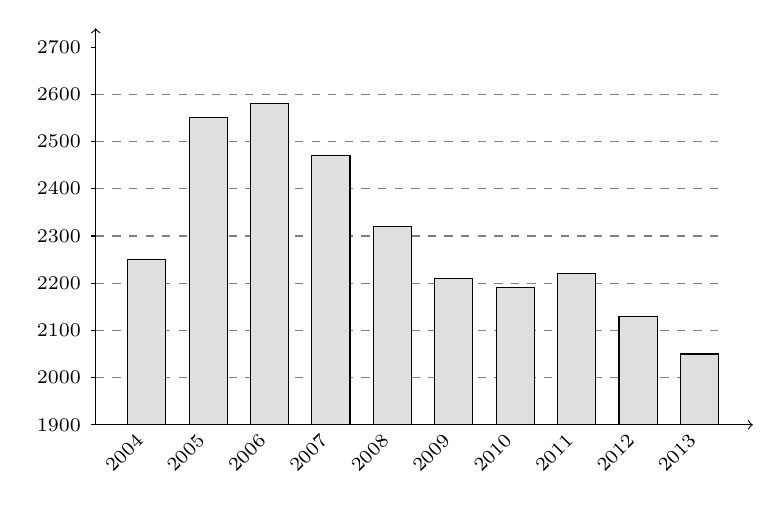
\begin{tikzpicture}[x=0.78cm,y=0.006cm,line width=0.4pt]
  % Approximate bar heights transcribed from the source image, not exact data.
  \draw[->] (0,1900) -- (10.7,1900);
  \draw[->] (0,1900) -- (0,2740);
  \foreach \y in {1900,2000,...,2700} {
    \draw (0,\y) -- (-0.08,\y) node[left] {\scriptsize \y};
  }
  \foreach \y in {2000,2100,...,2600} {
    \draw[dashed,gray] (0,\y) -- (10.2,\y);
  }
  \draw (0,1900) -- (10.2,1900);
  \foreach \i/\year/\v in {
    0/2004/2250,1/2005/2550,2/2006/2580,3/2007/2470,4/2008/2320,
    5/2009/2210,6/2010/2190,7/2011/2220,8/2012/2130,9/2013/2050} {
    \pgfmathsetmacro{\x}{0.52+\i}
    \draw[fill=gray!25] (\x,1900) rectangle ++(0.62,\v-1900);
    \node[below=2pt,rotate=45,anchor=east] at (\x+0.31,1900) {\scriptsize \year};
  }
\end{tikzpicture}
\end{center}
\nopagebreak[4]
(A) 逐年比较，2008 年减少二氧化硫排放量的效果最显著  
(B) 2007 年我国治理二氧化硫排放显现成效  
(C) 2006 年以来我国二氧化硫年排放量呈减少趋势  
(D) 2006 年以来我国二氧化硫年排放量与年份正相关

\Needspace{4\baselineskip}
\textbf{解析}

柱形图 2006 年附近最高，之后总体下降，2007 和 2008 连续显著下降；随年份增长总体排放减少，不能称正相关。2008 年的同比下降在图中最大。

\gkanswer{答案：D}

\end{answer}
\begin{answer}
\gksolhead{4}{}

\textbf{题目}：

已知 $\boldsymbol a=(1,-1)$，$\boldsymbol b=(-1,2)$，则 $(2\boldsymbol a+\boldsymbol b)\cdot\boldsymbol a=$（　）

(A) $-1$　(B) $0$　(C) $1$　(D) $2$

\Needspace{4\baselineskip}
\textbf{解析}

$2\boldsymbol a+\boldsymbol b=(1,0)$，与 $(1,-1)$ 点积为 $1$。

\gkanswer{答案：C，$1$}

\end{answer}
\begin{answer}
\gksolhead{5}{}

\textbf{题目}：

设 $S_n$ 是等差数列 $\{a_n\}$ 的前 $n$ 项和，若 $a_1+a_3+a_5=3$，则 $S_5=$（　）

(A) $5$　(B) $7$　(C) $9$　(D) $11$

\Needspace{4\baselineskip}
\textbf{解析}

等差数列 $a_1+a_3+a_5=3a_3=3$，故 $a_3=1$，$S_5=5a_3=5$。

\gkanswer{答案：A，$5$}

\end{answer}
\begin{answer}
\gksolhead{6}{}

\textbf{题目}：

一个正方体被一个平面截去一部分后，剩余部分的三视图如图，则截去部分体积与剩余部分体积的比值为（　）
\nopagebreak[4]
\begin{center}% FIG:q06-three-views
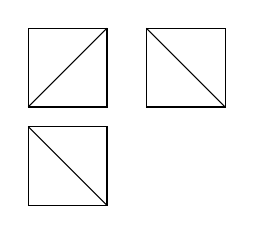
\begin{tikzpicture}[x=1cm,y=1cm,line width=0.4pt]
  \draw (0,1.25) rectangle (1,2.25);
  \draw (0,1.25) -- (1,2.25);
  \draw (1.5,1.25) rectangle (2.5,2.25);
  \draw (1.5,2.25) -- (2.5,1.25);
  \draw (0,0) rectangle (1,1);
  \draw (0,1) -- (1,0);
\end{tikzpicture}
\end{center}
\nopagebreak[4]
(A) $\dfrac18$　(B) $\dfrac17$　(C) $\dfrac16$　(D) $\dfrac15$

\Needspace{4\baselineskip}
\textbf{解析}

三个投影中切面斜线分别跨正方形对角，合起来对应在正方体一个顶点处截去三条互相垂直棱长均等于立方体棱长的角锥。设棱长为 $s$，截去的直角三棱锥体积为 $s^3/6$，余体积 $5s^3/6$，比值 $1/5$。此处形体重建是解题推导，不是原图明示的空间尺寸。

\gkanswer{答案：D，$\frac15$}

\end{answer}
\begin{answer}
\gksolhead{7}{}

\textbf{题目}：

已知三点 $A(1,0)$，$B(0,\sqrt3)$，$C(2,\sqrt3)$，则 $\triangle ABC$ 外接圆的圆心到原点的距离为（　）

(A) $\dfrac53$　(B) $\dfrac{\sqrt{21}}3$　(C) $\dfrac{2\sqrt5}3$　(D) $\dfrac43$

\Needspace{4\baselineskip}
\textbf{解析}

$BC$ 为水平弦，其垂直平分线为 $x=1$。设圆心 $(1,y)$，由到 $A,B$ 距离相等，$y^2=1+(y-\sqrt3)^2$，得 $y=2/\sqrt3$；距原点 $\sqrt{1+4/3}=\sqrt{21}/3$。

\gkanswer{答案：B，$\frac{\sqrt{21}}3$}

\end{answer}
\begin{answer}
\gksolhead{8}{}

\textbf{题目}：

下边程序框图的算法思路源于我国古代数学名著《九章算术》中的“更相减损术”。执行该程序框图，若输入的 $a,b$ 分别为 $14,18$，则输出的 $a=$（　）
\nopagebreak[4]
\begin{center}% FIG:q08-flowchart
\begin{tikzpicture}[>=stealth,line width=0.45pt,
  every node/.style={font=\small,align=center},
  terminal/.style={draw,rounded corners,minimum width=1.05cm,minimum height=0.48cm},
  io/.style={draw,minimum width=1.55cm,minimum height=0.5cm,shape=trapezium,trapezium left angle=70,trapezium right angle=110},
  decision/.style={draw,diamond,aspect=2.1,inner sep=1pt,minimum width=1.45cm,minimum height=0.7cm},
  process/.style={draw,minimum width=1.45cm,minimum height=0.48cm}]
  \node[terminal] (start) at (0,4.5) {开始};
  \node[io] (input) at (0,3.65) {输入 $a,b$};
  \node[decision] (neq) at (0,2.65) {$a\ne b$};
  \node[decision] (gt) at (0,1.25) {$a>b$};
  \node[io] (out) at (2.25,2.65) {输出 $a$};
  \node[terminal] (end) at (2.25,1.75) {结束};
  \node[process] (suba) at (-1.55,0.05) {$a=a-b$};
  \node[process] (subb) at (1.55,0.05) {$b=b-a$};
  \draw[->] (start) -- (input);
  \draw[->] (input) -- (neq);
  \draw[->] (neq.east) -- node[above]{否} (out.west);
  \draw[->] (out) -- (end);
  \draw[->] (neq.south) -- node[right]{是} (gt.north);
  \draw[->] (gt.south west) -- node[above left]{是} (suba.north);
  \draw[->] (gt.south east) -- node[above right]{否} (subb.north);
  \draw[->] (suba.south) -- (-1.55,-0.65);
  \draw[->] (subb.south) -- (1.55,-0.65);
  \draw (-1.55,-0.65) -- (1.55,-0.65);
  \draw[->] (-1.55,-0.65) -- (-3.6,-0.65) -- (-3.6,2.65) -- (neq.west);
\end{tikzpicture}
\end{center}
\nopagebreak[4]
(A) $0$　(B) $2$　(C) $4$　(D) $14$

\Needspace{4\baselineskip}
\textbf{解析}

框图不断从大数减去小数，保持最大公约数不变，最终 $a=b=\gcd(14,18)=2$，输出 $a=2$。

\gkanswer{答案：B，$2$}

\end{answer}
\begin{answer}
\gksolhead{9}{}

\textbf{题目}：

已知等比数列 $\{a_n\}$ 满足 $a_1=\dfrac14$，$a_3a_5=4(a_4-1)$，则 $a_2=$（　）

(A) $2$　(B) $1$　(C) $\dfrac12$　(D) $\dfrac18$

\Needspace{4\baselineskip}
\textbf{解析}

等比数列有 $a_3a_5=a_4^2$，令 $u=a_4$，则 $u^2=4(u-1)$，即 $(u-2)^2=0$，所以 $a_4=2$。由 $a_4=a_1q^3$ 得 $q^3=8$，$q=2$，$a_2=1/2$。

\gkanswer{答案：C，$\frac12$}

\end{answer}
\begin{answer}
\gksolhead{10}{}

\textbf{题目}：

已知 $A,B$ 是球 $O$ 的球面上两点，$\angle AOB=90^\circ$，$C$ 为该球面上的动点，若三棱锥 $O-ABC$ 体积的最大值为 $36$，则球 $O$ 的表面积为（　）

(A) $36\pi$　(B) $64\pi$　(C) $144\pi$　(D) $256\pi$

\Needspace{4\baselineskip}
\textbf{解析}

以 $OAB$ 为底，面积 $R^2/2$。球面点 $C$ 到其平面的最大距离为 $R$，所以最大体积 $R^3/6=36$，$R=6$，球面积 $4\pi R^2=144\pi$。

\gkanswer{答案：C，$144\pi$}

\end{answer}
\begin{answer}
\gksolhead{11}{}

\textbf{题目}：

如图，长方形 $ABCD$ 的边 $AB=2$，$BC=1$，$O$ 是 $AB$ 的中点，点 $P$ 沿着边 $BC,CD$ 与 $DA$ 运动，记 $\angle BOP=x$。将动点 $P$ 到 $A,B$ 两点距离之和表示为 $x$ 的函数 $f(x)$，则 $y=f(x)$ 的图象大致为（　）
\nopagebreak[4]
\begin{center}% FIG:q11-rectangle
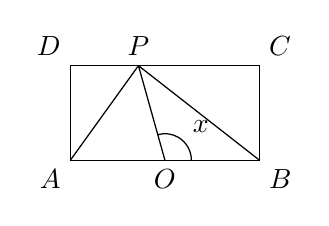
\begin{tikzpicture}[x=1.2cm,y=1.2cm,line width=0.45pt]
  \coordinate (A) at (0,0);
  \coordinate (B) at (2,0);
  \coordinate (C) at (2,1);
  \coordinate (D) at (0,1);
  \coordinate (O) at (1,0);
  \coordinate (P) at (0.72,1);
  \draw (A) -- (B) -- (C) -- (D) -- cycle;
  \draw (P) -- (A) (P) -- (O) (P) -- (B);
  \draw (A) node[below left] {$A$} (B) node[below right] {$B$}
    (C) node[above right] {$C$} (D) node[above left] {$D$}
    (O) node[below] {$O$} (P) node[above] {$P$};
  \draw (O) ++(0:0.28) arc[start angle=0,end angle=106,radius=0.28];
  \node at (1.38,0.36) {$x$};
\end{tikzpicture}
\end{center}
\nopagebreak[4]
\nopagebreak[4]
\begin{center}% FIG:q11-option-a
\begin{tikzpicture}[x=0.9cm,y=0.85cm,line width=0.45pt]
  \draw[->] (0,0) -- (4.45,0) node[right] {$x$};
  \draw[->] (0,0) -- (0,2.65) node[above] {$y$};
  \foreach \x/\lab in {1/{\frac{\pi}{4}},2/{\frac{\pi}{2}},3/{\frac{3\pi}{4}},4/{\pi}} {
    \draw (\x,0) -- +(0,-0.06) node[below=2pt] {$\lab$};
  }
  \draw (-0.07,2) -- (0.07,2) node[left=4pt] {$2$};
  \node[below left] at (0,0) {$O$};
  \draw (0,2) -- (1,2.48) -- (2,2.2) -- (3,2.48) -- (4,2);
\end{tikzpicture}
\end{center}
\nopagebreak[4]
\nopagebreak[4]
\begin{center}% FIG:q11-option-b
\begin{tikzpicture}[x=0.9cm,y=0.85cm,line width=0.45pt]
  \draw[->] (0,0) -- (4.45,0) node[right] {$x$};
  \draw[->] (0,0) -- (0,2.65) node[above] {$y$};
  \foreach \x/\lab in {1/{\frac{\pi}{4}},2/{\frac{\pi}{2}},3/{\frac{3\pi}{4}},4/{\pi}} {
    \draw (\x,0) -- +(0,-0.06) node[below=2pt] {$\lab$};
  }
  \draw (-0.07,2) -- (0.07,2) node[left=4pt] {$2$};
  \node[below left] at (0,0) {$O$};
  \draw (0,2) .. controls (0.35,2.35) and (0.78,2.60) .. (1,2.55)
    .. controls (1.08,2.25) and (1.65,2.05) .. (2,2.1)
    .. controls (2.35,2.05) and (2.88,2.20) .. (3,2.55)
    .. controls (3.2,2.60) and (3.65,2.35) .. (4,2);
\end{tikzpicture}
\end{center}
\nopagebreak[4]
\nopagebreak[4]
\begin{center}% FIG:q11-option-c
\begin{tikzpicture}[x=0.9cm,y=0.85cm,line width=0.45pt]
  \draw[->] (0,0) -- (4.45,0) node[right] {$x$};
  \draw[->] (0,0) -- (0,2.65) node[above] {$y$};
  \foreach \x/\lab in {1/{\frac{\pi}{4}},2/{\frac{\pi}{2}},3/{\frac{3\pi}{4}},4/{\pi}} {
    \draw (\x,0) -- +(0,-0.06) node[below=2pt] {$\lab$};
  }
  \draw (-0.07,2) -- (0.07,2) node[left=4pt] {$2$};
  \node[below left] at (0,0) {$O$};
  \draw (0,2) -- (2,2.52) -- (4,2);
\end{tikzpicture}
\end{center}
\nopagebreak[4]
\nopagebreak[4]
\begin{center}% FIG:q11-option-d
\begin{tikzpicture}[x=0.9cm,y=0.85cm,line width=0.45pt]
  \draw[->] (0,0) -- (4.45,0) node[right] {$x$};
  \draw[->] (0,0) -- (0,2.65) node[above] {$y$};
  \foreach \x/\lab in {1/{\frac{\pi}{4}},2/{\frac{\pi}{2}},3/{\frac{3\pi}{4}},4/{\pi}} {
    \draw (\x,0) -- +(0,-0.06) node[below=2pt] {$\lab$};
  }
  \draw (-0.07,2) -- (0.07,2) node[left=4pt] {$2$};
  \node[below left] at (0,0) {$O$};
  \draw (0,2) arc[start angle=180,end angle=0,x radius=2cm,y radius=0.55cm];
\end{tikzpicture}
\end{center}
\nopagebreak[4]
\Needspace{4\baselineskip}
\textbf{解析}

取 $A=(0,0),B=(2,0),C=(2,1),D=(0,1),O=(1,0)$。$P=B,A$ 时距离和均为 $2$；在顶边中点 $P=(1,1)$ 时为 $2\sqrt2$；在顶角 $C,D$ 时为 $1+\sqrt5>2\sqrt2$。沿 $BC$ 上升，沿 $CD$ 先降后升，沿 $DA$ 下降，因此两侧高峰、中间低谷且曲线在各边内部平滑，符合图 (B)。

\gkanswer{答案：B}

\end{answer}
\begin{answer}
\gksolhead{12}{}

\textbf{题目}：

设函数 $f(x)=\ln(1+|x|)-\dfrac1{1+x^2}$，则使得 $f(x)>f(2x-1)$ 成立的 $x$ 的取值范围是（　）

(A) $\left(\dfrac13,1\right)$　(B) $\left(-\infty,\dfrac13\right)\cup(1,+\infty)$  
(C) $\left(-\dfrac13,\dfrac13\right)$　(D) $\left(-\infty,-\dfrac13\right)\cup\left(\dfrac13,+\infty\right)$

\Needspace{4\baselineskip}
\textbf{解析}

令 $g(t)=\ln(1+t)-1/(1+t^2)$，$t\ge0$，则 $g'(t)=1/(1+t)+2t/(1+t^2)^2>0$。故原不等式等价于 $|x|>|2x-1|$，平方化为 $3x^2-4x+1<0$，即 $1/3<x<1$。

\gkanswer{答案：A，$(\frac13,1)$}

\end{answer}
\begin{answer}
\gksolhead{13}{}

\textbf{题目}：

已知函数 $f(x)=ax^3-2x$ 的图象过点 $(-1,4)$，则 $a=$\gkblank{}。

\Needspace{4\baselineskip}
\textbf{解析}

$f(-1)=-a+2=4$，故 $a=-2$。

\gkanswer{答案：$-2$}

\end{answer}
\begin{answer}
\gksolhead{14}{}

\textbf{题目}：

若 $x,y$ 满足约束条件 $\begin{cases}x+y-5\le0,\\2x-y-1\ge0,\\x-2y+1\le0,\end{cases}$ 则 $z=2x+y$ 的最大值为\gkblank{}。

\Needspace{4\baselineskip}
\textbf{解析}

可行域的顶点由三对边界线相交得 $(1,1),(2,3),(3,2)$；对应 $z=3,7,8$，最大值为 $8$。

\gkanswer{答案：$8$}

\end{answer}
\begin{answer}
\gksolhead{15}{}

\textbf{题目}：

已知双曲线过点 $(4,\sqrt3)$，且渐近线方程为 $y=\pm\dfrac12x$，则该双曲线的标准方程为\gkblank{}。

\Needspace{4\baselineskip}
\textbf{解析}

渐近线斜率为 $1/2$。若双曲线以 $x$ 为实轴，则 $b^2=a^2/4$，由点 $(4,\sqrt3)$ 在曲线上得 $16/a^2-3/b^2=1$，所以 $a^2=4,b^2=1$。以 $y$ 为实轴的代入会得负的轴平方，舍去。

\gkanswer{答案：$\frac{x^2}{4}-y^2=1$}

\end{answer}
\begin{answer}
\gksolhead{16}{}

\textbf{题目}：

已知曲线 $y=x+\ln x$ 在点 $(1,1)$ 处的切线与曲线 $y=ax^2+(a+2)x+1$ 相切，则 $a=$\gkblank{}。

\Needspace{4\baselineskip}
\textbf{解析}

$y=x+\ln x$ 在 $x=1$ 处导数为 $2$，切线 $y=2x-1$。另一曲线与此线相切，需 $ax^2+ax+2=0$ 有重根；$a\ne0$ 且判别式 $a^2-8a=0$，故 $a=8$。

\gkanswer{答案：$8$}

\end{answer}
\begin{answer}
\gksolhead{17}{}

\textbf{题目}：

$\triangle ABC$ 中，$D$ 是 $BC$ 上的点，$AD$ 平分 $\angle BAC$，$BD=2DC$。

(1) 求 $\dfrac{\sin\angle B}{\sin\angle C}$；  
(2) 若 $\angle BAC=60^\circ$，求 $\angle B$。

\Needspace{4\baselineskip}
\textbf{解析}

\gksubpart{(1)}

角平分线定理给 $AB/AC=BD/DC=2$，由正弦定理 $AB/AC=\sin C/\sin B$，故所求比为 $1/2$。

\gksubpart{(2)}

当 $A=60^\circ$，$C=120^\circ-B$。由 $2\sin B=\sin(120^\circ-B)$ 得 $\tan B=1/\sqrt3$，结合 $0<B<120^\circ$ 得 $B=30^\circ$。

\gkanswer{答案（1）：$\frac12$}

\gkanswer{答案（2）：$30^\circ$}

\end{answer}
\begin{answer}
\gksolhead{18}{}

\textbf{题目}：

某公司为了了解用户对其产品的满意度，从 $A,B$ 两地区分别随机调查了 $40$ 个用户，根据用户对其产品的满意度的评分，得到 $A$ 地区用户满意度评分的频率分布直方图和 $B$ 地区用户满意度评分的频率分布表。

$A$ 地区用户满意度评分的频率分布直方图：
\nopagebreak[4]
\begin{center}% FIG:q18-a-histogram
\begin{tikzpicture}[x=0.105cm,y=115cm,line width=0.4pt]
  \draw[->] (36,0) -- (106,0) node[right] {满意度评分};
  \draw[->] (40,0) -- (40,0.044) node[above] {频率/组距};
  \foreach \x in {40,50,...,100} {
    \draw (\x,0) -- +(0,-0.00035) node[below=2pt] {\scriptsize \x};
  }
  \foreach \y/\label in {0.005/0.005,0.010/0.010,0.015/0.015,0.020/0.020,0.025/0.025,0.030/0.030,0.035/0.035,0.040/0.040} {
    \draw (40,\y) -- +(1.0,0);
    \node[left=4pt] at (40,\y) {\scriptsize \label};
  }
  \foreach \y in {0.005,0.015,0.020,0.030} {
    \draw[dashed,gray] (40,\y) -- (100,\y);
  }
  \foreach \l/\r/\h in {40/50/0.010,50/60/0.020,60/70/0.030,70/80/0.020,80/90/0.015,90/100/0.005} {
    \draw (\l,0) rectangle (\r,\h);
  }
\end{tikzpicture}
\end{center}
\nopagebreak[4]
$B$ 地区用户满意度评分的频率分布表：

\begin{center}
\begin{tabular}{lrrrrr}
\toprule
满意度评分分组 & $[50,60)$ & $[60,70)$ & $[70,80)$ & $[80,90)$ & $[90,100]$ \\
\midrule
频数 & 2 & 8 & 14 & 10 & 6 \\
\bottomrule
\end{tabular}
\end{center}

(1) 在图中作出 $B$ 地区用户满意度评分的频率分布直方图，并通过此图比较两地区满意度评分的平均值及分散程度；（不要求计算出具体值，给出结论即可）
\nopagebreak[4]
\begin{center}% FIG:q18-b-blank-grid
\begin{tikzpicture}[x=0.12cm,y=115cm,line width=0.35pt]
  \draw[->] (45,0) -- (106,0) node[right] {满意度评分};
  \draw[->] (50,0) -- (50,0.044) node[above] {频率/组距};
  \foreach \x in {50,60,...,100} {
    \draw (\x,0) -- (\x,0.040);
    \draw (\x,0) -- +(0,-0.00035) node[below=2pt] {\scriptsize \x};
  }
  \foreach \y/\label in {0.005/0.005,0.010/0.010,0.015/0.015,0.020/0.020,0.025/0.025,0.030/0.030,0.035/0.035,0.040/0.040} {
    \draw (50,\y) -- (100,\y);
    \node[left=4pt] at (50,\y) {\scriptsize \label};
  }
\end{tikzpicture}
\end{center}
\nopagebreak[4]
(2) 根据用户满意度评分，将用户的满意度评分分为三个等级：

\begin{center}
\begin{tabular}{llll}
\toprule
满意度评分 & 低于 $70$ 分 & $70$ 分到 $89$ 分 & 不低于 $90$ 分 \\
\midrule
满意度等级 & 不满意 & 满意 & 非常满意 \\
\bottomrule
\end{tabular}
\end{center}

估计哪个地区的用户的满意度等级为不满意的概率大，说明理由。

\Needspace{4\baselineskip}
\textbf{解析}

\gksubpart{(1)}

B 地区各组频率/组距为频数除以 $40\times10$，依次 $0.005,0.020,0.035,0.025,0.015$，应在原空白网格的 $50$–$100$ 五组上作柱。A 地区柱高依次为 $0.010,0.020,0.030,0.020,0.015,0.005$（$40$–$100$ 六组）。从分布位置及离散幅度看，B 地区平均评分更高，A 地区更分散。若用组中值作检算，平均值约为 A $67.5$、B $77.5$；这一计算只作独立核验，原题不要求具体值。
\nopagebreak[4]
\begin{center}% 2015 全国Ⅱ文科 18(1) 解答图：B 地区频率分布直方图。
% 对照源卷第 968 页空白网格；横轴保留 40 左端界及 50--100 刻度，纵轴至 0.040。
\begin{tikzpicture}[font=\small, x=0.105cm, y=125cm]
  % 原卷网格（仅绘图区域，不复录题干）。
  \foreach \x in {40,50,...,100}
    \draw[gray!65, line width=0.25pt] (\x,0) -- (\x,0.04);
  \foreach \y in {0.005,0.010,...,0.040}
    \draw[gray!65, line width=0.25pt] (40,\y) -- (100,\y);

  % 五组柱高为频率/组距：0.005、0.020、0.035、0.025、0.015。
  \foreach \left/\right/\height in {
      50/60/0.005,
      60/70/0.020,
      70/80/0.035,
      80/90/0.025,
      90/100/0.015}
    \filldraw[fill=gray!18, draw=black, line width=0.55pt]
      (\left,0) rectangle (\right,\height);

  % 坐标轴与刻度。
  \draw[-stealth, line width=0.65pt] (40,0) -- (103,0);
  \draw[-stealth, line width=0.65pt] (40,0) -- (40,0.0435);
  \foreach \x in {50,60,...,100} {
    \draw (\x,0) -- (\x,-0.00065);
    \node[below, inner sep=2pt] at (\x,-0.00065) {\footnotesize \x};
  }
  \foreach \y/\label in {
      0.005/0.005,
      0.010/0.010,
      0.015/0.015,
      0.020/0.020,
      0.025/0.025,
      0.030/0.030,
      0.035/0.035,
      0.040/0.040} {
    \draw (40,\y) -- (39.2,\y);
    \node[left, inner sep=2pt] at (39.2,\y) {\footnotesize \label};
  }
  \node[below left, inner sep=1.5pt] at (40,0) {$O$};
  \node[right, inner sep=3pt] at (103,0) {满意度评分};
  \node[above, inner sep=2pt] at (40,0.0435) {频率/组距};
\end{tikzpicture}
\end{center}
\nopagebreak[4]
\gksubpart{(2)}

不满意即低于 70 分，A 的估计概率为 $(0.010+0.020+0.030)\times10=0.60$，B 为 $(2+8)/40=0.25$，故 A 地区较大。

\gkanswer{答案（1）：B 地各组柱高为 $0.005,0.020,0.035,0.025,0.015$；B 地平均值较高、分散较小}

\gkanswer{答案（2）：A 地较大（A 地 $0.60$，B 地 $0.25$）}

\end{answer}
\begin{answer}
\gksolhead{19}{}

\textbf{题目}：

如图，长方体 $ABCD-A_1B_1C_1D_1$ 中，$AB=16$，$BC=10$，$AA_1=8$，点 $E,F$ 分别在 $A_1B_1,D_1C_1$ 上，$A_1E=D_1F=4$。过点 $E,F$ 的平面 $\alpha$ 与此长方体的面相交，交线围成一个正方形。

(1) 在图中画出这个正方形（不必说明画法和理由）；  
(2) 求平面 $\alpha$ 把该长方体分成的两部分体积的比值。
\nopagebreak[4]
\begin{center}% FIG:q19-cuboid
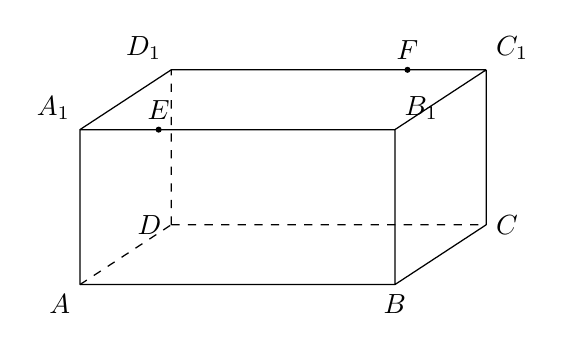
\begin{tikzpicture}[x={(1cm,0cm)},y={(0.58cm,0.38cm)},z={(0cm,0.82cm)},line width=0.45pt]
  \coordinate (A) at (0,0,0);
  \coordinate (B) at (4,0,0);
  \coordinate (C) at (4,2,0);
  \coordinate (D) at (0,2,0);
  \coordinate (Aone) at (0,0,2.4);
  \coordinate (Bone) at (4,0,2.4);
  \coordinate (Cone) at (4,2,2.4);
  \coordinate (Done) at (0,2,2.4);
  \coordinate (E) at (1,0,2.4);
  \coordinate (F) at (3,2,2.4);
  \draw (A)--(B)--(C) (A)--(Aone)--(Bone)--(B) (Bone)--(Cone) (Cone)--(C)
    (Aone)--(Done)--(Cone) (Done)--(F) (Aone)--(E);
  \draw[dashed] (A)--(D) (D)--(C) (D)--(Done);
  \foreach \p/\pos/\lab in {A/below left/A,B/below/B,C/right/C,D/left/D,Aone/above left/{A_1},Bone/above right/{B_1},Cone/above right/{C_1},Done/above left/{D_1},E/above/{E},F/above/{F}} {
    \node[\pos] at (\p) {$\lab$};
  }
  \fill (E) circle (1.1pt);
  \fill (F) circle (1.1pt);
\end{tikzpicture}
\end{center}
\nopagebreak[4]
\Needspace{4\baselineskip}
\textbf{解析}

取 $A=(0,0,0),B=(16,0,0),D=(0,10,0),A_1=(0,0,8)$，则 $E=(4,0,8),F=(4,10,8)$，$EF=10$。要使截面成正方形，从 $E,F$ 向另一侧各取长为 $10$ 的斜边，竖直差为 $8$、水平差为 $6$。

\gksubpart{(1)}

在 $AB,DC$ 上分别取 $H=(10,0,0),K=(10,10,0)$，连接 $E-H-K-F-E$。四边长均为 $10$，且相邻边垂直，故为所求正方形。$H,K$ 是解答所作点，原题图不预画截面。
\nopagebreak[4]
\begin{center}% 2015 全国Ⅱ文科 19(1) 解答图。斜投影按源卷第 966 页盒体前后方向：
% 前面为 y=0，后面为 y=10；EH 与 KF 按要求以虚线表示遮挡段。
% 方形边界 HK、KF、FE、EH 是解答新增线，题面原盒体图不含这些线。
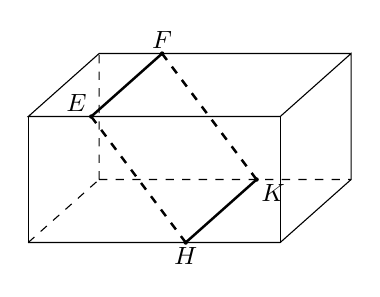
\begin{tikzpicture}[
  font=\small,
  x={(0.20cm,0cm)},
  y={(0.09cm,0.08cm)},
  z={(0cm,0.20cm)}
]
  % 长方体各顶点及题目所给截面点。
  \coordinate (A)  at (0,0,0);
  \coordinate (B)  at (16,0,0);
  \coordinate (C)  at (16,10,0);
  \coordinate (D)  at (0,10,0);
  \coordinate (A1) at (0,0,8);
  \coordinate (B1) at (16,0,8);
  \coordinate (C1) at (16,10,8);
  \coordinate (D1) at (0,10,8);
  \coordinate (E)  at (4,0,8);
  \coordinate (F)  at (4,10,8);
  \coordinate (H)  at (10,0,0);
  \coordinate (K)  at (10,10,0);

  % 源盒体外轮廓；被前面遮挡的后底边与后左竖边用虚线。
  \draw (A)--(B)--(C)--(C1)--(B1)--(A1)--(D1)--(C1);
  \draw (A)--(A1) (B)--(B1);
  \draw[dashed] (A)--(D) (D)--(C) (D)--(D1);

  % 解答新增的正方形 E-H-K-F；EH、KF按解答图的遮挡约定画为虚线。
  \draw[dashed, line width=0.9pt] (E)--(H);
  \draw[line width=0.9pt] (H)--(K);
  \draw[dashed, line width=0.9pt] (K)--(F);
  \draw[line width=0.9pt] (F)--(E);

  \foreach \pt in {E,F,H,K}
    \fill (\pt) circle (0.8pt);
  \node[above left, inner sep=1.5pt] at (E) {$E$};
  \node[above, inner sep=1.5pt] at (F) {$F$};
  \node[below, inner sep=1.5pt] at (H) {$H$};
  \node[below right, inner sep=1.5pt] at (K) {$K$};
\end{tikzpicture}
\end{center}
\nopagebreak[4]
\gksubpart{(2)}

截面平面为 $z=\frac43(10-x)$。对固定 $y$，$0\le x\le4$ 部分全高为 $8$，体积截面积为 $4\cdot8$；$4\le x\le10$ 部分为底 $6$、高 $8$ 的三角形。沿 $y$ 方向长度为 $10$，左侧体积为 $10[4\cdot8+\frac12\cdot6\cdot8]=560$。长方体总积 $16\cdot10\cdot8=1280$，另一侧为 $720$，故两部分体积比为 $7:9$。

\gkanswer{答案（1）：在 $AB,DC$ 上取 $H,K$，$AH=DK=10$，连接 $EHKF$}

\gkanswer{答案（2）：两部分体积比为 $7:9$（或逆序 $9:7$）}

\end{answer}
\begin{answer}
\gksolhead{20}{}

\textbf{题目}：

已知椭圆 $C:\dfrac{x^2}{a^2}+\dfrac{y^2}{b^2}=1$（$a>b>0$）的离心率为 $\dfrac{\sqrt2}2$，点 $(2,\sqrt2)$ 在 $C$ 上。

(1) 求 $C$ 的方程；  
(2) 直线 $l$ 不经过原点 $O$，且不平行于坐标轴，$l$ 与 $C$ 有两个交点 $A,B$，线段 $AB$ 中点为 $M$，证明：直线 $OM$ 的斜率与直线 $l$ 的斜率乘积为定值。

\Needspace{4\baselineskip}
\textbf{解析}

\gksubpart{(1)}

$e^2=1-b^2/a^2=1/2$，所以 $b^2=a^2/2$。代入 $(2,\sqrt2)$：$4/a^2+2/b^2=8/a^2=1$，故 $C:x^2/8+y^2/4=1$。

\gksubpart{(2)}

设 $A=(x_1,y_1),B=(x_2,y_2),M=(x_m,y_m)$，由两点椭圆方程相减，$x_m(x_1-x_2)/4+y_m(y_1-y_2)/2=0$。令直线 $l$ 斜率 $k=(y_1-y_2)/(x_1-x_2)$，则 $x_m/4+k y_m/2=0$，即 $k\cdot(y_m/x_m)=-1/2$。在所给非原点、非坐标轴平行条件下相关斜率有定义，故定值为 $-1/2$。

\gkanswer{答案（1）：$\frac{x^2}{8}+\frac{y^2}{4}=1$}

\gkanswer{答案（2）：$-\frac12$}

\end{answer}
\begin{answer}
\gksolhead{21}{}

\textbf{题目}：

已知 $f(x)=\ln x+a(1-x)$。

(1) 讨论 $f(x)$ 的单调性；  
(2) 当 $f(x)$ 有最大值，且最大值大于 $2a-2$ 时，求 $a$ 的取值范围。

\Needspace{4\baselineskip}
\textbf{解析}

定义域 $x>0$，$f'(x)=1/x-a$。

\gksubpart{(1)}

当 $a\le0$ 时在 $(0,+\infty)$ 严格递增；当 $a>0$ 时在 $(0,1/a)$ 递增、在 $(1/a,+\infty)$ 递减。

\gksubpart{(2)}

仅 $a>0$ 时有最大值，$f(1/a)=-\ln a+a-1$。要求 $-\ln a+a-1>2a-2$，即 $1-a-\ln a>0$。左式在 $a>0$ 上严格递减，在 $a=1$ 为零，故 $0<a<1$。

\gkanswer{答案（1）：$a\le0$ 时递增；$a>0$ 时在 $(0,1/a)$ 递增、$(1/a,+\infty)$ 递减}

\gkanswer{答案（2）：$0<a<1$}

\end{answer}
\begin{answer}
\gksolhead{22}{}

\textbf{题目}：

如图，$O$ 为等腰三角形 $ABC$ 内一点，$\odot O$ 与 $\triangle ABC$ 的底边 $BC$ 交于 $M,N$ 两点，与底边上的高 $AD$ 交于点 $G$，且与 $AB,AC$ 分别相切于 $E,F$ 两点。

(1) 证明：$EF\parallel BC$；  
(2) 若 $AG$ 等于 $\odot O$ 的半径，且 $AE=MN=2\sqrt3$，求四边形 $EBCF$ 的面积。
\nopagebreak[4]
\begin{center}% FIG:q22-triangle-circle
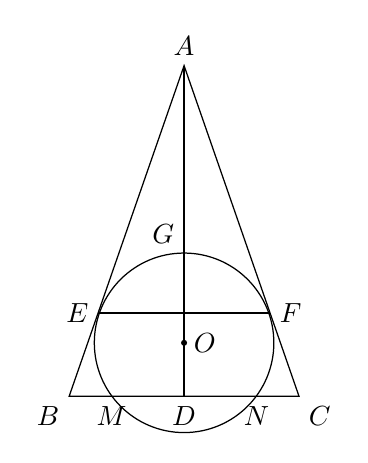
\begin{tikzpicture}[x=1cm,y=1cm,line width=0.45pt]
  \coordinate (A) at (0,4.2);
  \coordinate (B) at (-1.46,0);
  \coordinate (C) at (1.46,0);
  \coordinate (D) at (0,0);
  \coordinate (O) at (0,0.68);
  \coordinate (E) at (-1.09,1.06);
  \coordinate (F) at (1.09,1.06);
  \coordinate (G) at (0,1.82);
  \coordinate (M) at (-0.92,0);
  \coordinate (N) at (0.92,0);
  \draw (A)--(B)--(C)--cycle;
  \draw (0,4.2)--(0,0);
  \draw (O) circle[radius=1.14];
  \draw (E)--(F);
  \fill (O) circle (1.1pt);
  \foreach \p/\pos/\lab in {A/above/A,B/below left/B,C/below right/C,D/below/D,O/right/O,E/left/E,F/right/F,G/above left/G,M/below/M,N/below/N} {
    \node[\pos] at (\p) {$\lab$};
  }
\end{tikzpicture}
\end{center}
\nopagebreak[4]
\Needspace{4\baselineskip}
\textbf{解析}

\gksubpart{(1)}

圆同时切等腰三角形两腰，其圆心在顶角平分线 $AD$ 上。由圆外一点切线长，$AE=AF$；又 $AB=AC$，所以 $AE/AB=AF/AC$，由比例逆定理 $EF\parallel BC$。

\gksubpart{(2)}

设圆半径 $r$、$OD=k$、$AD=h$、$BD=DC=s$。$G$ 是图示上方交点，$AG=h-k-r=r$，故 $h-k=2r$。切线长 $AE^2=AO^2-r^2=3r^2$，由 $AE=2\sqrt3$ 得 $r=2$；弦长 $MN=2\sqrt{r^2-k^2}=2\sqrt3$，$O$ 在底边上方，故 $k=1,h=5$。三角形腰所在直线与圆相切，距离公式给 $r=(h-k)s/\sqrt{s^2+h^2}$，代入得 $2=4s/\sqrt{s^2+25}$，所以 $s=5/\sqrt3$，$BC=10/\sqrt3$、$AB=10/\sqrt3$。由 $AE/AB=3/5$，相似三角形 $AEF\sim ABC$ 的高为 $3h/5=3$，故四边形 $EBCF$ 高为 $2$、上底 $EF=(3/5)BC=2\sqrt3$。面积 $\frac12(BC+EF)\cdot2=16\sqrt3/3$。

\gkanswer{答案（1）：$EF\parallel BC$，见证明}

\gkanswer{答案（2）：$\frac{16\sqrt3}{3}$}

\end{answer}
\begin{answer}
\gksolhead{23}{}

\textbf{题目}：

在直角坐标系 $xOy$ 中，曲线 $C_1:\begin{cases}x=t\cos\alpha,\\y=t\sin\alpha,\end{cases}$（$t$ 为参数，$t\ne0$），其中 $0\le\alpha<\pi$。在以 $O$ 为极点，$x$ 轴正半轴为极轴的极坐标系中，曲线 $C_2:\rho=2\sin\theta$，$C_3:\rho=2\sqrt3\cos\theta$。

(1) 求 $C_2$ 与 $C_3$ 交点的直角坐标；  
(2) 若 $C_1$ 与 $C_2$ 相交于点 $A$，$C_1$ 与 $C_3$ 相交于点 $B$，求 $|AB|$ 的最大值。

\Needspace{4\baselineskip}
\textbf{解析}

\gksubpart{(1)}

$C_2$ 化为 $x^2+y^2=2y$，$C_3$ 化为 $x^2+y^2=2\sqrt3x$。相减得 $y=\sqrt3x$，代入得 $x=0$ 或 $\sqrt3/2$，因此交点为 $(0,0)$ 与 $(\sqrt3/2,3/2)$。

\gksubpart{(2)}

对非原点交点，$C_1$ 上的有向参数分别为 $t_A=2\sin\alpha$，$t_B=2\sqrt3\cos\alpha$；$t=0$ 被题设排除，故实际相交时两者须非零。距离 $|AB|=|t_A-t_B|=2|\sin\alpha-\sqrt3\cos\alpha|\le4$。取 $\alpha=5\pi/6$ 时两交点均非原点，等号成立，故 最大值 $4$。

\gkanswer{答案（1）：$(0,0)$、$(\frac{\sqrt3}{2},\frac32)$}

\gkanswer{答案（2）：$4$（$\alpha=5\pi/6$ 时取到，两交点均有定义）}

\end{answer}
\begin{answer}
\gksolhead{24}{}

\textbf{题目}：

设 $a,b,c,d$ 均为正数，且 $a+b=c+d$，证明：

(1) 若 $ab>cd$，则 $\sqrt a+\sqrt b>\sqrt c+\sqrt d$；  
(2) $\sqrt a+\sqrt b>\sqrt c+\sqrt d$ 是 $|a-b|<|c-d|$ 的充要条件。

\Needspace{4\baselineskip}
\textbf{解析}

记共同的和为 $S=a+b=c+d>0$。

\gksubpart{(1)}

$(\sqrt a+\sqrt b)^2=S+2\sqrt{ab}$，$(\sqrt c+\sqrt d)^2=S+2\sqrt{cd}$。由 $ab>cd$ 且两边正，即得 $\sqrt a+\sqrt b>\sqrt c+\sqrt d$。

\gksubpart{(2)}

上述平方比较说明根式和严格大当且仅当 $ab>cd$。另一方面 $|a-b|^2=S^2-4ab$、$|c-d|^2=S^2-4cd$，故 $ab>cd$ 当且仅当 $|a-b|<|c-d|$。两端同为严格不等式，充分性和必要性均成立。

\gkanswer{答案（1）：命题成立，见证明}

\gkanswer{答案（2）：两条件互为充要条件，见证明}

\end{answer}